
\chapter{正多面体与五次方程解}




\section{引入:从正多面体至分歧覆叠}
我们从最熟悉的对象——正多面体着手.

经典理论告诉我们3维欧式空间中的正多面体只有5种,其基本性质见下表:

%Automorphism of dodecahedron is $S_2 \times A_5$, not $S_5$.
\begin{table}[ht]
	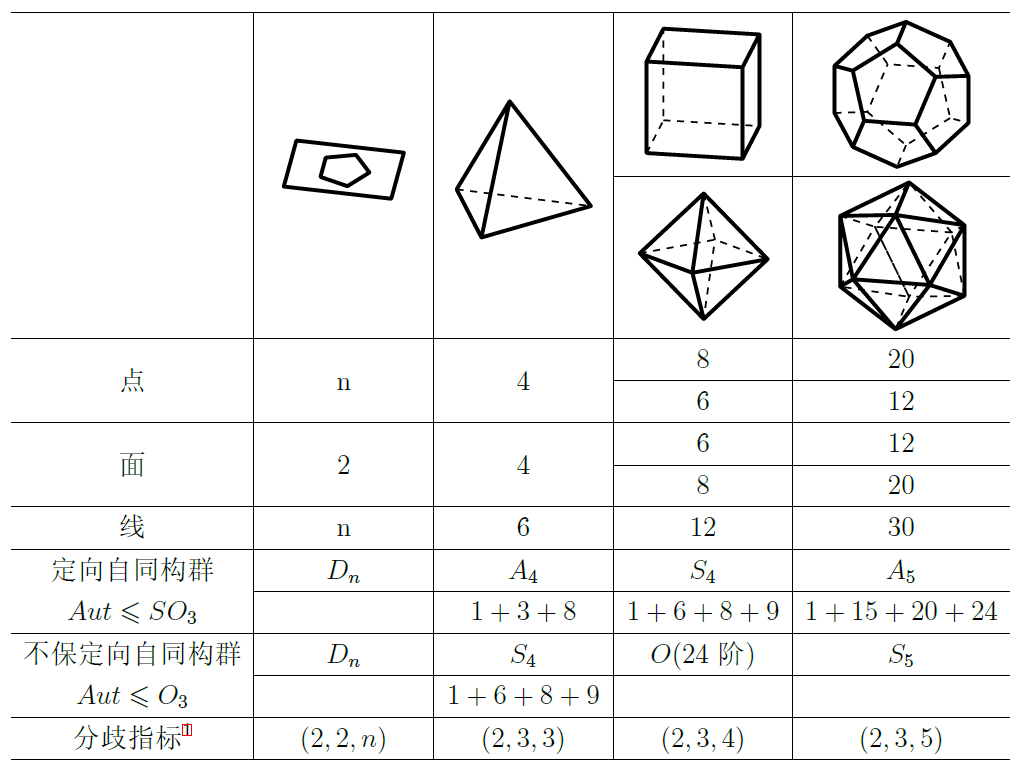
\includegraphics[width=0.98\textwidth]{snip/propofpoly.png}
\end{table}

	正多面体的重要性在于对称性,故必然引入群的概念.将其表面投影至球面$S^2=\mathbb{P}\mathbb{C}^1$,注意到$S^2$的等距自同构群为$SO_3\cong \mathbb{P}SU_2 \cong\mathbb{R}\mathbb{P}^3$,我们有交换图表:
\begin{figure}[ht]
	\centering
	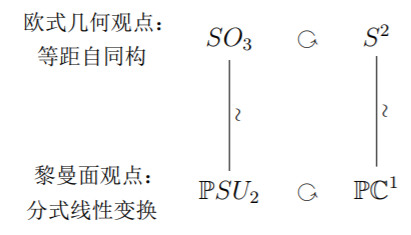
\includegraphics[]{snip/tikz-iso.png}
\end{figure}
		
		
		则正多面体的等距自同构群自然同构于$SO_3$ 的某个离散子群,记作$\Gamma$.另一方面,由\cite[5.9.1]{artin2011algebra}或\cite[2.6]{shurman1997geometry}知旋转群$SO_3$的离散子群除$\mathbb{Z}/n\mathbb{Z}$外只有上图给出的这几种;由\cite{shurman1997geometry},任一个$\Aut (\mathbb{PC}^1)$的有限子群必共轭于$SO_3$的子群,从而被清晰归类.
		

		在抽象代数中,我们已经掌握了这些群的代数性质.但现在我们再从几何/群作用的观点加深理解.
		
		\begin{enumerate}
			\item 	首先, $SO_3$的任何一个元素可以用以下方式表示:
			\begin{itemize}
				\item 	$3\times3$实矩阵;
				\item 	$2\times2$酉矩阵(作为分式线性变换)\footnote{注意$A$和$-A$表示同一个作用,我们将发展更丰富的理论来弥补这个``缺陷",如双多面体群.};
				\item 	绕某个轴旋转:\raisebox{-0.25cm}{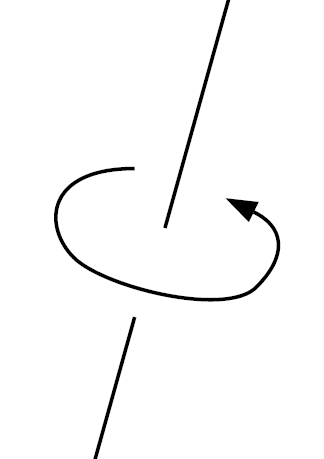
\includegraphics[width=0.5cm]{pic/rotaion.png}} (+$Id$)
			\end{itemize}
			这意味着每个$SO_3$的离散子群也可以用上述方式表示.\footnote{离散子群作为分式线性变换的表示,参见\cite[p46-47]{klein2003lectures}}.
			\item  其次, $\Gamma$在正多面体上的作用诱导了在正多面体的点、线、面上的作用.
			
			\item
			$\Gamma$ 在$S^2$上的作用,诱导了$\Gamma$ 在基本区域上的作用,这个作用是忠实且满的,即对任意基本区域$D_1,D_2$,存在唯一$\gamma\in\Gamma$使得$\gamma D_1=D_2$.所谓基本区域如下定义:
			\begin{defn}[基本区域]
				设$\Gamma$为$SO_3$的离散子群,称开集$D\subseteq S^2$为($S^2$相对于) $\Gamma$的\textbf{基本区域},如果:
				
				\begin{itemize}
					\item 对任意$\gamma\in\Gamma\smallsetminus\{Id\}$, $\gamma(D)\cap D=\varnothing$;
					
					\item $S^2=\bigcup_{\gamma\in\Gamma}\overline{\gamma(D)}$.
				\end{itemize}
			\end{defn}
		容易画出$\Gamma$的基本区域,例如图\ref{pic:basicdis}的红色区域.基于对称性,往后只考虑形如右图或者其平移的基本区域. 该图形的形状规则,可以省去很多不必要的麻烦.
			\begin{figure}[ht]
					%正十二面体
					\centering
					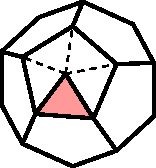
\includegraphics[]{poly/poly4-1.pdf}
					\caption{正十二面体群的基本区域}
					\label{pic:basicdis}
			\end{figure}
		\begin{exercise}
	利用基本区域计算$\Gamma$的阶. (可直接计数/求基本区域与$S^2$的面积比)
\end{exercise}

\item  既然群$\Gamma$作用于集合$S^2$,我们有轨道集$S^2/\Gamma$.在拓扑上,由右图可以看出$S^2/\Gamma\overset{\sim}{\longrightarrow}S^2$.
以Riemann曲面的观点,在赋予$S^2/\Gamma$标准的复结构之后,商映射$S^2\xtwoheadrightarrow{} S^2/\Gamma$可视作Riemann曲面之间的分歧覆叠
$$\varPhi:\mathbb{PC}^1\xtwoheadrightarrow{}\mathbb{PC}^1/\Gamma\overset{\sim}{\longrightarrow}\mathbb{PC}^1$$
该映射可视作$\mathbb{C}$上的有理函数\footnote{这些有理函数均可计算,见表\ref{tb:equations}}.
\begin{figure}[ht]
	
	\begin{minipage}[t]{.34\textwidth}
		\vspace{0.1cm}
		%正十二面体
		\centering
		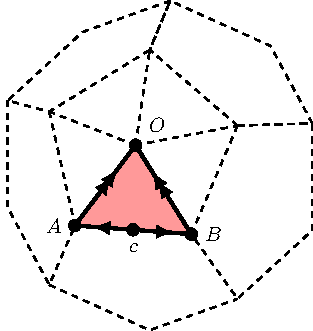
\includegraphics[width=3cm]{poly/poly4-2.pdf}
		
	\end{minipage}
	\begin{minipage}[t]{.64\textwidth}
		\vspace{0.1cm}
		\centering
		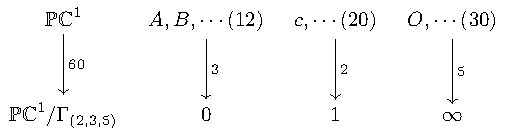
\includegraphics[]{commu/commu2.pdf}
		\caption*{在$0,1,\infty$处分歧,分歧指标为$(2,3,5)$}
	\end{minipage}
	\caption{例:正十二面体}
	\label{pic:comm2}
\end{figure}

\begin{exercise}
	写出(或画出)以上分歧覆叠的分歧点与对应的分歧指标,如图\ref{pic:comm2}.
\end{exercise}

为方便起见,我们用分歧指标作为下标来标记正多面体的定向自同构群,如$\Gamma_{(2,3,5)}$为正十二面体的定向自同构群.\footnote{该群作为$SO_3$的子群,依赖于正多面体在空间中的摆放位置,习惯上固定了正多面体的位置.}
\end{enumerate}


这些多面体之间同样有趣味的关系:
\begin{figure}[ht]
		\begin{minipage}[t]{.28\textwidth}
		\centering
		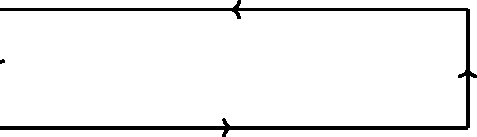
\includegraphics[scale=0.8]{poly/poly24.pdf}
		\caption{}
		\label{eg:fig1}
	\end{minipage}
	\begin{minipage}[t]{.22\textwidth}
		\centering
		%正方体套三角锥
		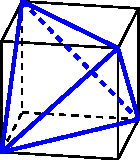
\includegraphics[]{poly/poly12.pdf}
		\caption{}
		\label{eg:fig2}
	\end{minipage}
	\begin{minipage}[t]{.22\textwidth}
		\centering
		%正方体套对角线
		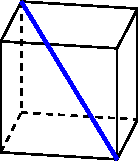
\includegraphics[]{poly/poly001.pdf}
		\caption{}
		\label{eg:fig3}
	\end{minipage}
	\begin{minipage}[t]{.22\textwidth}
		\centering
		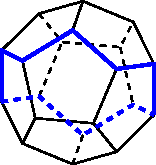
\includegraphics[]{poly/poly04.pdf}
		\caption{}
		\label{eg:fig4}
	\end{minipage}
\end{figure}

\begin{example1}\
		\begin{itemize}
			\item 图\ref{eg:fig1}给出$\Gamma_{(2,3,5)}$的一个12阶子群$A_4$;
			
			\item 不同的正方体给出不同且互相共轭的12阶子群;
			
			\item $\Gamma_{(2,3,5)}$中的元素给出5个正方体的置换,即群同态$\alpha:\Gamma_{(2,3,5)}\longrightarrow S_5$.易验证$\ker(\alpha)=\{Id\}$, $Im(\alpha)=A_5$.因此$\Gamma_{(2,3,5)}\cong A_5$.
			
		\end{itemize}
	
\end{example1}
\begin{example1}
		同上,图\ref{eg:fig2}给出$\Gamma_{(2,3,4)}$的6阶子群$A_4$及群同态$\Gamma_{(2,3,4)}\longrightarrow S_2$.
\end{example1}
\begin{example1}		
		同上,图\ref{eg:fig3}给出$\Gamma_{(2,3,4)}$的4个互相共轭的6阶子群$D_3$及群同态$\Gamma_{(2,3,4)}\longrightarrow S_4$.由此可得$\Gamma_{(2,3,4)}\cong S_4$.
\end{example1}
\begin{example1}
		同上,图\ref{eg:fig4}给出$\Gamma_{(2,3,4)}$的4个互相共轭的6阶子群$D_3$及群同态$\Gamma_{(2,3,4)}\longrightarrow S_4$.由此可得$\Gamma_{(2,3,4)}\cong S_4$.
\end{example1}


\begin{exercise}
	写出(或画出)以上分歧覆叠的分歧点与对应的分歧指数.这些分歧覆叠均可视作有理函数且可计算,可查阅表\ref{tb:equations}.
\end{exercise}

从态射的角度,对$\Aut (\mathbb{P}\mathbb{C}^1)$的两个离散子群$H \subseteq G$,我们能得到分歧覆叠$\mathbb{P}\mathbb{C}^1/H \xtwoheadrightarrow{} \mathbb{P}\mathbb{C}^1/G$.我们可以画出/写出分歧点与对应的分歧指标,给出该覆叠所对应的有理函数.\footnote{部分覆叠所对应的有理函数,见表2.在第\ref{sec:inverse-alge}节我们会使用更方便的方法来计算这些有理函数.}

作为抽象理论的补充,我们以一个具体的例子来结束本小结.

\begin{exercise}
	给定群嵌入$\Gamma_{(2,3,3)}\xhookrightarrow{\quad}\Gamma_{(2,3,5)}$,尝试计算分歧覆叠$\mathbb{PC}^1/\Gamma_{(2,3,3)}\xtwoheadrightarrow{}\mathbb{PC}^1/\Gamma_{(2,3,5)}$ 的信息.
\end{exercise}
\begin{proof}
	为方便起见,调整$\mathbb{PC}^1/\Gamma_{(2,3,3)}$的基本区域为一个五边形,如图\ref{fig:tran}.通过对图\ref{fig:tran}的观察,得到分歧指标如图
	\ref{fig:ramify1}.
	
	
	
	\begin{figure}[ht]
		\begin{minipage}[t]{.25\textwidth}
			\vspace{0cm}
			\centering
			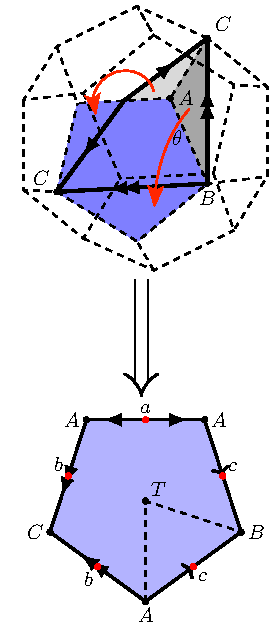
\includegraphics[width=3cm]{planet/planet5.pdf}
			\caption{}
			\label{fig:tran}
		\end{minipage}
		\begin{minipage}[t]{.65\textwidth}
			\vspace{0cm}
			\centering
			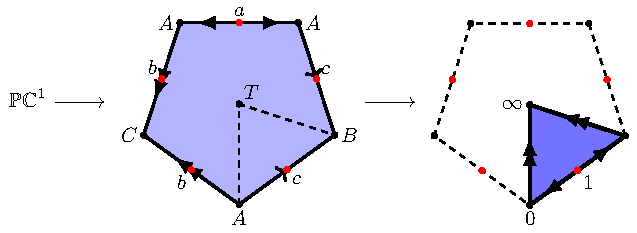
\includegraphics[width=9cm]{planet/planet3.pdf}
			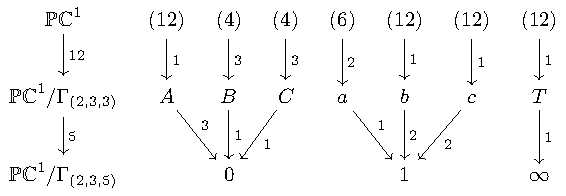
\includegraphics[]{commu/commu1.pdf}
			\caption{分歧点与分歧指标}
			\label{fig:ramify1}
		\end{minipage}
		
	\end{figure}
	
	
	
	
	
	现在我们来求该覆叠所对应的有理函数$Z(r)$.
	
	取
	$$\gamma:\mathbb{PC}^1/\Gamma_{(2,3,3)}\overset{\sim}{\longrightarrow}\mathbb{PC}^1\qquad T\longmapsto\infty,\;a\longmapsto0,\;A\longmapsto\alpha$$ 其中$\alpha\in\mathbb{R}\smallsetminus\{0\}$为待定参数.
	\begin{itemize}
		\item 由Schwarz反射原理, $\gamma(B)=\overline{\gamma(C)}:=z_0$, $\gamma(b)=\overline{\gamma(c)}$.
		\item $Z(r)$为5次多项式, $Z(0)=1,Z(\alpha)=Z(z_0)=Z(\overline{z_0})=0$.
		
		\item $Z(r)=c(r-\alpha)^3(r^2-\beta r+\gamma),\quad\beta,\gamma\in\mathbb{R}$.这蕴含$c=-\frac{1}{\alpha^3\gamma}\in\mathbb{R} \smallsetminus \{0\}$.
	\end{itemize}
	
	调节$\alpha$使得$c=-1/1728$\footnote{取$\alpha=1$后得到$c$的值,重新取$\alpha=-(1728c)^{\frac{1}{5}}$即可.},则
	$$Z:Z-1:1\;=\;(r-\alpha)^3(r^2-\beta r+\gamma):r(r^2-\epsilon r+\xi)^2:-1728,$$
	其中$\alpha,\beta,\gamma,\epsilon,\xi\in\mathbb{R}$.上式蕴含
	\begin{equation}
	(r\alpha)^3(r^2-\beta r+\gamma)+1728=r(r^2-\epsilon r+\xi)^2.
	\end{equation}
	
	对比$r$的次数展开后,这个方程组有$5$个变量, $5$个方程,看似已无解.但是,所谓“山重水复疑无路,柳暗花明又一村”,在\textbf{奇妙}的消元法之后,我们得到
	\[Z:Z-1:1\;=\;(r-3)^3(r^2-11r+64):r(r^2-10r+45)^2:-1728.\]
	
	下面简要陈述这个奇妙的消元法,摘自\cite[P111]{klein2003lectures}.
	
	在(0.1)式两边求导,得到
	$$(r-\alpha)^2\big(5r^2-(2\alpha+4\beta)r+(\alpha\beta+3\gamma)\big)=(r^2-\epsilon r+\xi)(5r^2-3\epsilon r+\xi). $$
	但由于$b,c\neq a$,故$(r-\alpha)$与$(r^2-\epsilon r+\xi)$互素,故有方程组
	$$\begin{cases}5\epsilon=2\alpha+4\beta\\5\xi=\alpha\beta+3\gamma\\10\alpha=3\epsilon\\5\alpha^2=\xi\end{cases}$$
	依次消去$\epsilon,\xi,\beta$得到$64a^2=9\gamma$;对(0.1)式取$r=0$得$\alpha^3\gamma=1728$.综合两式,我们有$a^5=3^5$,由$a\in\mathbb{R}$知$a=3$.其余参数均容易顺次求出.
	\begin{exercise}\label{exercise:function}
		利用分歧映射以及上文给出的映射$\gamma$,说明覆叠$\mathbb{P}\mathbb{C}^1 \longrightarrow \mathbb{P}\mathbb{C}^1/\Gamma_{(2,3,3)}$所对应的有理函数$r(z)$可记为$\frac{t^2(z)}{f(z)}$,其中$t(z)$为6次多项式,在立方体的面心各有一个1阶零点; $f(z)$为12次多项式,于正十二面体的面心处各有一个1阶零点.
	\end{exercise}
	
\end{proof}
\section{综述}
上一节中,我们从正多面体的对称性出发,导出分歧覆叠
$$\varPhi\colon \mathbb{PC}^1 \xrightarrow{\qquad} \mathbb{PC}^1/\Gamma \cong \mathbb{PC}^1$$
%数学中对逆映射特别在意,在这里也是:
%\begin{center}
%	\fbox
%	{给定$Z \in \mathbb{C}$,尝试赋予$\varPhi^{-1}(Z)$恰当的定义,并描述$\varPhi^{-1}(Z)$的性质.}
%\end{center}
在第\ref{sec:inva}节,我们将利用不变量理论给出$\Phi$的表达式.在第\ref{sec:inverse-comp},\ref{sec:inverse-alge}节,我们将以复分析/近世代数的方式研究$\Phi^{-1}$.在最后,我们将研究如何用模形式/正十二面体方程来解一般的五次方程. 整个流程图如下:
\begin{figure}[ht]
	
	\begin{minipage}[t]{.9\textwidth}
		\vspace{0.1cm}
		\centering
		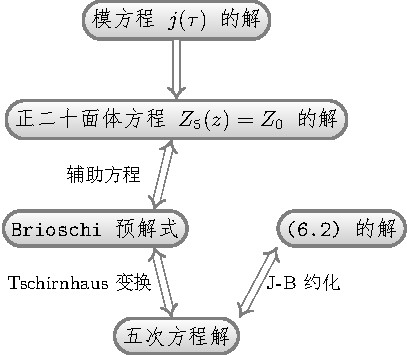
\includegraphics{Flowchart/Mainflowchart.pdf}
		
	\end{minipage}
	\label{pic:flow}
\end{figure}
\section[不变量理论]{不变量理论\protect\footnote{本节主要参考了\cite[Chapter 3]{shurman1997geometry}.}}\label{sec:inva}

	在本节中,记$\mathbb{C}_n\homopoly$为$n$次齐次多项式构成的集合, $\mathbb{C}\homopoly:= \bigcup_{n=0}^{+\infty} \mathbb{C}_n\homopoly$为齐次多项式构成的集合,注意$\mathbb{C}_n[z_1,z_2]$与$\mathbb{C}_n\homopoly$的区别.记$f\sim g \Leftrightarrow $存在$k \in \mathbb{C}^*$, $f=kg$.习惯性称齐次多项式为形式(form)\footnote{这是因为$n$次齐次多项式可视作$\mathcal{O}_{\mathbb{PC}^1}(n)$的一个全纯截影.}. 

\subsection{不变函数与半不变量}
函数空间(层)是几何对象的灵魂.直觉来看, $X/G$上的函数可视为$X$上满足对称性($f(\gamma z)= f(z)$)的函数\footnote{然而这不是常态. $X/G$可能是很怪异的空间(如$\mathbb{P}^2/PGL_2$,见\cite[Example 10.8]{mumford1995algebraic}),函数空间的选取也需要足够合适.但对于有限群在代数簇上的作用,商空间总是存在并构成一个代数簇,见\cite{mumford1995algebraic}.},这使得不变量理论进入了我们的视野:
\begin{defn}
	设有限群$\Gamma$作用在$\mathbb{PC}^1$上.称亚纯函数$f$为$\Gamma$-\textbf{不变函数},若对任意$\gamma \in \Gamma, z \in \mathbb{PC}^1$,
	$$f(\gamma z)=f(z)$$
\end{defn}
在黎曼面课上我们知道,任一个$\mathbb{PC}^1$上的亚纯函数$f$可视作两个互质多项式$G,H\in \mathbb{C}\homopoly$的比\footnote{今后均假设$G,H$互质.}:
$$f\big(\homopoly\big)=\big[G(z_1,z_2):H(z_1,z_2)\big], \quad\text{ 简记为 } \,f=[G:H]$$
这使我们想要探索$\Gamma$与$\mathbb{C}\homopoly$的关系.定义
$$\Gamma':= \left\{ A \in SU_2 \mid \bar{A} \in \Gamma \right\}$$
为群$\Gamma$的提升,则
\begin{itemize}
	\item $\Gamma' \subseteq SU_2$作用在$\mathbb{C}\homopoly$上$\left( \begin{bmatrix}
	a & b \\ c & d
	\end{bmatrix} (z_1,z_2):= (az_1+bz_2:cz_1+dz_2) \right)$
	\item $|\Gamma'|=2|\Gamma|$, $\Gamma$为有限群;
	\item 记$\gamma' \in \Gamma'$为$\gamma \in \Gamma$的提升,则
	$$f \circ \gamma = [G \circ \gamma' : H \circ \gamma']$$
\end{itemize}
\begin{defn}
	称形式$F$以$\bigchi_F: \Gamma' \longrightarrow \mathbb{C}^*$为特征的$\Gamma'$-\textbf{半不变量},若对任意$\gamma' \in \Gamma'$,
	$$F\big(\gamma' \homopoly\big)=\bigchi_F(\gamma')\, F\big(\homopoly\big),\quad \text{ 简记为 } \,F \circ \gamma'= \bigchi_F(\gamma') F. $$
	当$\bigchi_F$平凡时,我们称形式$F$为$\Gamma$-不变量.
\end{defn}
容易看出,若$G,H \in \mathbb{C}_n\homopoly$均为以$\bigchi$为特征的$\Gamma'$-半不变量,则$f=[G:H]$为$\Gamma$-不变函数.令人惊奇的是,反之也是成立的:
\begin{theorem}[{\cite[Proposition 3.1.2]{shurman1997geometry}}]\label{thm:repofinvfunc}
	设亚纯函数$f=[G:H]$为$\Gamma$-不变函数,则存在特征$\bigchi \in \Hom_{Grp}(\Gamma', \mathbb{C}^*)$,使得$G,H$为以$\bigchi$为特征的$\Gamma'$-半不变量.
\end{theorem}
\begin{proof}
	直接的代数论证,见\cite[exercise 3.13]{shurman1997geometry}.
\end{proof}

这样我们将不变函数的问题转移到$\Gamma'$-半不变量上.我们将刻画所有的不变量,以及描述其中特殊元素之间的关系,从而得到它们的表达式.可以说,不变量理论是定量计算的有力武器.
\subsection{轨道形式}
我们知道, $\mathbb{PC}^1$上的全纯截影由其除子(记录截影零点的位置和阶数)唯一决定(忽略常数因子).记$\divi(f)=\sum_{\text{finite}}n_iP_i$,则$\divi(f\circ \gamma')=\sum_{\text{finite}}n_i\gamma'(P_i)$,故
\begin{equation*}
\begin{aligned}
&f\text{ 为 }\,\Gamma'\text{-半不变量}\\
\Leftrightarrow\,&\text{对任意}\,\gamma' \in \Gamma',\, \divi(f)=\divi(f \circ \gamma')\\
\Leftrightarrow\,& \divi(f)=\sum_{\text{i finite}} \sum_{P \in \mathcal{O}_i}P,\,\text{其中$\mathcal{O}_i$为$\Gamma$在$\mathbb{PC}^1$上的某个轨道.}\\
\end{aligned}
\end{equation*}
故$\Gamma'$-半不变量亦可被称作轨道形式(orbit form).

我们定义一类特殊的轨道形式,这类轨道形式可以有清晰的表达,并且具有相同的特征.回忆定理 \ref{thm:repofinvfunc},这给出了我们需要的$\Gamma$-不变函数.
\begin{defn}[全轨道形式]
	我们称$f \in \mathbb{C}_{|\Gamma|}\homopoly$为\textbf{全轨道形式},若存在轨道$\mathcal{O}_f$,使得
	$$\divi (f)= \frac{|\Gamma|}{|\mathcal{O}_f|} \sum_{P \in \mathcal{O}_f}P$$
\end{defn}

设$F_p$为以$p=[p_1,p_2]$为零点的全轨道形式,对每个$\gamma \in \Gamma$写成两个线性映射的商: $\gamma=\frac{\gamma_1}{\gamma_2}$,则
$$F_p(z_1,z_2) \sim \prod_{\gamma \in \Gamma}\left(\gamma_2(p_1,p_2)z_1-\gamma_1(p_1,p_2)z_2\right)$$
可以看出,固定$\gamma_0 \in \Gamma$, $\bigchi_{F_p}(\gamma_0)$是关于$p$良定义的连续函数,而$|\Gamma|$次单位根是离散空间,故$\bigchi_{F_p}(\gamma_0)$为常值函数,所有全轨道形式具有相同的特征,记为$\bigchi_{\Gamma}$.

对正多面体群\footnote{旋转群只在两个轨道处退化,这时理论只需略微修正,如令$F_3=z_1^n-z_2^n$.},全轨道形式恰好在三个轨道处(记为$\mathcal{O}_1,\mathcal{O}_2,\mathcal{O}_3$)退化\footnote{指$|\Gamma| \neq |\mathcal{O}_i|$.},成为某个非退化轨道形式的$v_i:=|\Gamma|/|\mathcal{O}_i|$次幂.我们写出这些非退化轨道形式:
$$F_i= \prod_{[p_1:p_2] \in \mathcal{O}_i}(p_2z_1-p_1z_2)$$
记所对应的特征为$\bigchi_i$.
\begin{example1}
	对旋转群$\Gamma=\mathbb{Z}/n\mathbb{Z} \curvearrowright \mathbb{PC}^1$,此时只有2个非平凡轨道:
	$$\mathcal{O}_1=\left\{[1:0] \right\} \qquad \mathcal{O}_2=\left\{[0:1] \right\}$$
	故$F_1=z_2$, $F_2=z_1$.(不在意常系数).对$s_{n}':=\begin{pmatrix}
	\omega_{2n} & 0 \\ 0 & \bar{\omega}_{2n}
	\end{pmatrix} \in \Gamma'$, 
	$$F_1 \circ \homopoly =F_1[\omega_{2n}z_1 : \bar{\omega}_{2n} z_2] = \bar{\omega}_{2n} z_2=\bar{\omega}_{2n} F_1$$
	故$$\bigchi_1:s_n' \longmapsto \bar{\omega}_{2n}, \quad -I \longmapsto -1. $$
	同理可证$\bigchi_2=\bar{\bigchi}_1$.当取$F_3=z_1^n-z_2^n$时, $\bigchi_3=\bigchi_{\Gamma}=\bigchi_1^n$.
\end{example1}
\begin{example1}
	对正二面体群$\Gamma=D_{n} \curvearrowright \mathbb{PC}^1$,此时三个轨道分别为
	\begin{equation*}
	\mathcal{O}_1=\left\{ [1:0], [0,1] \right\}, \quad
	\mathcal{O}_2=\left\{ [\omega_{n}^a:1] \big| a \in \mathbb{Z} \right\}, \quad
	\mathcal{O}_3=\left\{ [\omega_{2n}\omega_{n}^a:1] \big| a \in \mathbb{Z} \right\} .
	\end{equation*}
	得到三个半不变量
	$$F_1=z_1z_2, \quad F_2=\frac{z_1^n-z_2^n}{2}, \quad F_3=\frac{z_1^n+z_2^n}{2}. $$
	记$s_{n}':=\begin{pmatrix}
	\omega_{2n} & 0 \\ 0 & \bar{\omega}_{2n}
	\end{pmatrix}$, $t':=\begin{pmatrix}
	0 & i \\ i & 0
	\end{pmatrix} \in \Gamma'$, 通过计算得到
	\begin{equation*}
	\begin{aligned}
	&\bigchi_1:s_n' \longmapsto \phantom{-}1, \quad t' \longmapsto -1\\
	&\bigchi_2:s_n' \longmapsto -1, \quad t' \longmapsto i^n \qquad \bigchi_3=\bar{\bigchi}_2
	\end{aligned}
	\end{equation*}
\end{example1}
下面这个定理告诉我们,这些特殊的轨道形式给出了所有(全)轨道形式的表达:(特殊蕴含一般)
\begin{theorem}[{\cite[Theorem 3.3.2, Exercise 3.2.3]{shurman1997geometry}}]\label{thm:expr} 任一个全轨道形式均可以表达为$F=\lambda_1F_1^{v_1}+\lambda_2F_2^{v_2}$, $\lambda=[\lambda_1,\lambda_2] \in \mathbb{PC}^1$的形式.
	
	任一个轨道形式均可以表达为
	$$F=F_1^{e_1}F_2^{e_2}F_3^{e_3}\prod_{\substack{\lambda=[\lambda_1:\lambda_2]\\\text{finite}}}(\lambda_1F_1^{v_1}+\lambda_2F_2^{v_2})^{e_{\lambda}},\qquad 0 \leqslant e_i < v_i$$
	的形式.
	
	这些表达在忽略常系数的情况下唯一.
\end{theorem}
\begin{proof}
	只需观察(全)轨道形式的零点位置即可.
\end{proof}
\begin{corollary}
	$F_1,F_2,F_3$之间存在唯一的代数关系:
	$$c_1F_1^{v_1}-c_2F_2^{v_2}+c_3F_3^{v_3}=0$$
\end{corollary}
这时已可以用暴力列举法来算$F_i$了,但计算仍然繁杂.通过协变函子的帮助,可以由$F_1$推出$F_2$和$F_3$.在此之前,我们以正二十面体的$F_1$的计算为例,来说明$F_1$的计算方式.
\begin{example1}[正二十面体的$F_1$]
	写出正十二面体的面点(即是正二十面体的顶点)对应的轨道
	$$\mathcal{O}_1:=\left\{0,\infty,\omega_5^i\varphi,-\omega_5^i\varphi^{-1} \right\}$$
	得到
	\begin{equation*}
	\begin{aligned}
	F_1 = \,& z_1z_2 \prod_{i=0}^{4}(z_1-\omega_5^i\varphi z_2) \prod_{i=0}^{4}(z_1+\omega_5^i\varphi^{-1} z_2) \\
	= \,& z_1z_2(z_1^5-\varphi^5 z_2^5)(z_1^5+\varphi^{-5}z_2^5)\\
	= \,& z_1z_2(z_1^{10}-(\varphi^5-\varphi^{-5})z_1^5z_2^5-z_2^{10})\\
	= \,& z_1z_2(z_1^{10}+11z_1^5z_2^5-z_2^{10})\\
	\end{aligned}
	\end{equation*}
	由于$A_5$是非交换单群,故无非平凡1维表示.
\end{example1}
\subsection{协变函子$H$, $J$}
\begin{defn}
	我们称协变函子$C: \mathbb{C} \homopoly \longrightarrow \mathbb{C} \homopoly$与$\Gamma'$相容,若存在$e\in \mathbb{Z}$,使得对任意$\gamma' \in \Gamma'$, $a \in \mathbb{C}^*$, $F \in \mathbb{C} \homopoly$,有
	$$C(F \circ \gamma')= C(F) \circ \gamma' \qquad C(aF)=a^eC(F)$$
	当$F$为以$\bigchi_F$为特征的$\Gamma'$-不变量时, $C(F)$为以$\bigchi_F^e$为特征的$\Gamma'$-不变量.
\end{defn}
\begin{example1}
	对$\Gamma'$-不变量,定义Hesse函子$H$与Jacobi函子$J$:
	$$M_H(F)= \begin{bmatrix}
	D_{11}F & D_{12}F \\ D_{21}F & D_{22}F 
	\end{bmatrix} 	\qquad H=\det M_H$$
	$$M_J(F)= \begin{bmatrix}
	D_{1}F & D_{1}HF \\D_{2}F & D_{2}HF
	\end{bmatrix} 	\qquad J=\det M_J$$
	经过繁复的计算, $H$, $J$均与$\Gamma'$相容,并且
	$$\deg (HF)=2(\deg F-2), \quad \deg(JF)=3(\deg F-2),$$
	$$ \quad \bigchi_{HF}=\bigchi_F^2, \quad \bigchi_{JF}=\bigchi_F^3. $$
\end{example1}
\begin{proof}
	按顺序计算$D_i(F \circ \gamma')$, $D_{ij}(F \circ \gamma')$, $H(F \circ \gamma')$, $J(F \circ \gamma')$:
	
	\begin{flalign*}
	D_i(F \circ \gamma') = & D_i\big(F(a_{11}z_1+a_{12}z_2,a_{21}z_1+a_{22}z_2) \big)&\\                                                                 
	= & \sum_{k \in \{1,2\}} a_{ki} (D_kF) \circ \gamma'\footnotemark &
	\end{flalign*}
	\footnotetext{矩阵表示可以让我们对今后的计算看得更清楚:
		$$\begin{bmatrix}
		D_1(F \circ \gamma') \\ D_2(F \circ \gamma')
		\end{bmatrix}=
		\begin{bmatrix}
		a_{11} & a_{21} \\ a_{12} & a_{22}
		\end{bmatrix}
		\begin{bmatrix}
		D_1F \circ \gamma' \\ D_2F \circ \gamma'
		\end{bmatrix}
		$$}
	\begin{flalign*}
	D_{ij}(F \circ \gamma') = &	D_i \big[D_j (F \circ \gamma') \big]				&\\
	= &	D_i\left[\sum_{l}a_{lj}(D_lF) \circ \gamma' \right]						&\\
	= &\sum_{l}a_{lj}D_i \big[(D_lF) \circ \gamma'\big]							&\\
	= &	\sum_{l}a_{lj}\left[\sum_k a_{ki} (D_kD_lF) \circ \gamma'\right]						&\\
	= &	\sum_{k,l} a_{ki} (D_{kl}F) \circ \gamma' a_{lj}						&
	\end{flalign*}
	\begin{flalign*}
	H(F \circ \gamma')= &	\det \begin{bmatrix}
	D_{11}(F \circ \gamma') & D_{12}(F \circ \gamma') \\
	D_{12}(F \circ \gamma') & D_{22}(F \circ \gamma')
	\end{bmatrix}						&\\	
	= &	\det \left( \begin{bmatrix}
	a_{11} & a_{21} \\ a_{12} & a_{22}
	\end{bmatrix}
	\begin{bmatrix}
	(D_{11}F) \circ \gamma' & (D_{12}F) \circ \gamma' \\
	(D_{21}F) \circ \gamma' & (D_{22}F) \circ \gamma'
	\end{bmatrix}
	\begin{bmatrix}
	a_{11} & a_{12} \\ a_{21} & a_{22}
	\end{bmatrix}\right)						&\\
	= &	\det \begin{bmatrix}
	(D_{11}F) \circ \gamma' & (D_{12}F) \circ \gamma' \\
	(D_{21}F) \circ \gamma' & (D_{22}F) \circ \gamma'
	\end{bmatrix}						&\\
	= &	H(F) \circ \gamma'						&
	\end{flalign*}
	\begin{flalign*}	
	J(F \circ \gamma')	= &	\det	\begin{bmatrix}
	D_1(F \circ \gamma') & D_1H(F \circ \gamma') \\
	D_2(F \circ \gamma') & D_2H(F \circ \gamma')
	\end{bmatrix}					&\\	
	= &	\det \begin{bmatrix}
	D_1(F \circ \gamma') & D_1(HF \circ \gamma') \\
	D_2(F \circ \gamma') & D_2(HF \circ \gamma')
	\end{bmatrix}						&\\
	= &	\det \left( \begin{bmatrix}
	a_{11} & a_{21} \\ a_{12} & a_{22}
	\end{bmatrix}
	\begin{bmatrix}
	(D_{1}F)\circ \gamma' & (D_{1}HF)\circ \gamma' \\
	(D_{2}F)\circ \gamma' & (D_{2}HF)\circ \gamma'
	\end{bmatrix}
	\right)						&\\
	= &	(JF) \circ \gamma'						&	
	\end{flalign*}
	其余论断均显然.
\end{proof}

通过对次数的比照,运用定理\ref{thm:expr},以及一点额外的计算,我们惊奇地发现\footnote{我怀疑这里可以用$H$, $J$的几何直观看出,但我没有证据.},对非退化的正多面体群(亦即,除$C_n$, $D_n$外), $F_2=H(F_1)$, $F_3=J(F_1)$.这样我们得到了所有有限群对应的$F_1,F_2,F_3$以及之间的代数关系,如图\ref{tb:equations}.可以说,到目前为止,我们对$\mathbb{PC}^1$上的不变量理论有了一个较为彻底的理解.
\subsection{结论汇总}
	\begin{table}[ht]
		\centering
		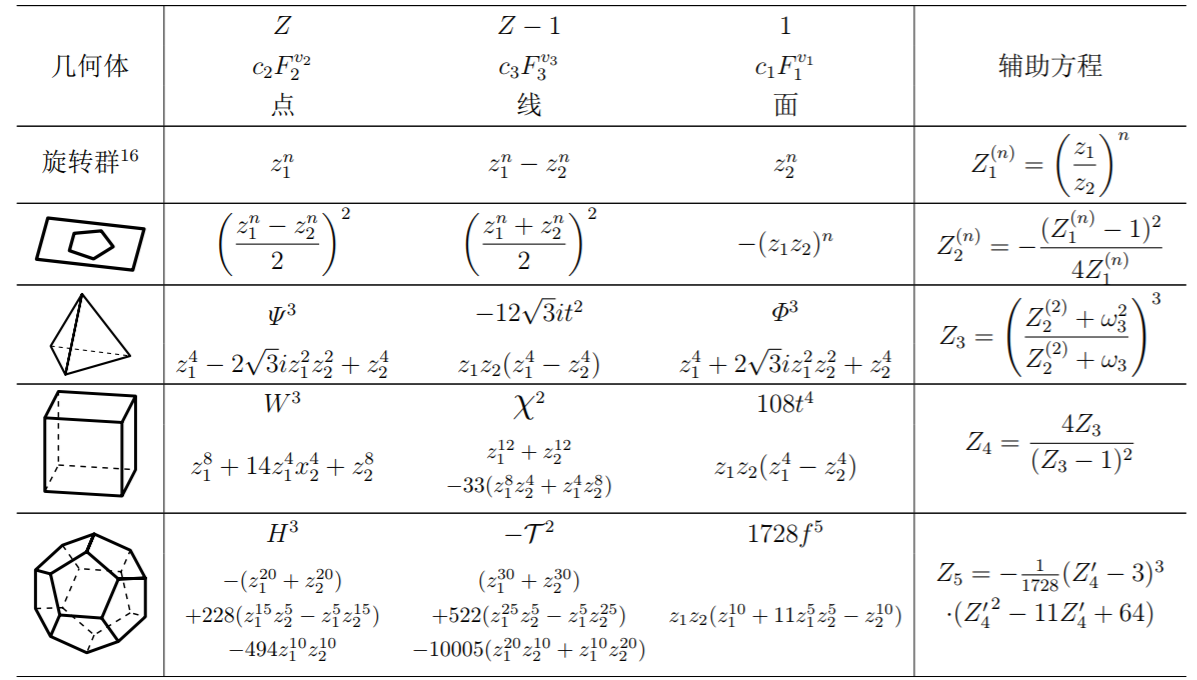
\includegraphics[width=0.98\textwidth]{snip/eqpoly.png}
	\caption{正多面体对应方程}
	\label{tb:equations}
\end{table}
\footnotetext{$Z_1^{(n)}$不对应几何体, $v_1 \neq 2$ !}

\begin{remarks}\
	\begin{enumerate}[1.]
		\item 由于嵌入正十二面体的立方体为倾斜放置,辅助方程为$Z_4'$,与$Z_4$相差一个分式线性变换.倾斜的立方体对应的$F_1,F_2,F_3$及其代数关系如下:
	\begin{figure}[ht]
	\centering
	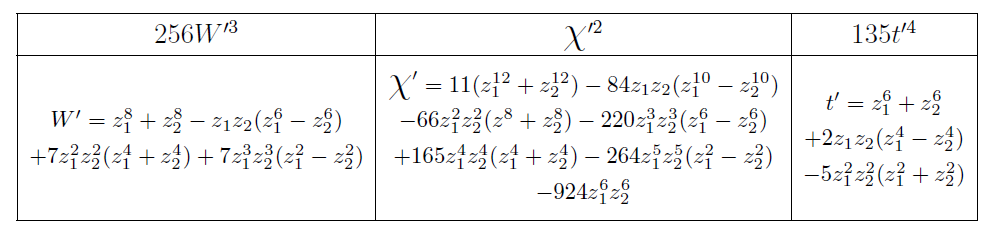
\includegraphics[width=0.98\textwidth]{snip/slantpoly.png}
\end{figure}
		\item 通过辅助方程,除$Z_5(z)$以外的其他方程均可解出,且为根式解.但是正十二面体所对应的最后一个辅助方程是5次方程,运用Galois的理论我们得到该方程的不可解性.我们将在第\ref{sec:inverse-alge}节中具体解释该现象.
	\end{enumerate}
\end{remarks}
返回看我们最初的问题,我们可以轻而易举地写出一个非常值的$\Gamma$-不变函数:
$$Z:= \frac{c_2F_2^{v_2}}{c_1F_1^{v_1}}$$
这可看作是黎曼面$\mathbb{PC}^1/\Gamma$上的一个亚纯函数,由于$\mathbb{PC}^1/\Gamma \cong \mathbb{PC}^1$,故$\mathbb{PC}^1/\Gamma$上的亚纯函数空间是$\mathbb{C}(Z) = \mathbb{C}(z)^{\Gamma}$.从代数的角度,这个等式可以从对例外轨道形式的描述中得到,详见\cite[3.5,3.6]{shurman1997geometry}.
\begin{remarks}\
	\begin{enumerate}
		\item 如何定义商空间$\mathbb{PC}^1/\Gamma$的代数簇结构?这里我们讨论的是$\Gamma'$-半不变量,当考虑对应的$\Gamma’$-不变量(平凡特征)时,不变量代数$\mathbb{C}[z_1,z_2]^{\Gamma'}$所对应的射影概型$\Proj\mathbb{C}[z_1,z_2]^{\Gamma'}$即为所求的商空间.注意这里作为代数簇, $$\Proj\mathbb{C}[z_1,z_2]^{\Gamma'} = \mathbb{PC}^1//\Gamma \neq \mathbb{PC}^1.$$
		\item  有了坐标环,我们可以发掘新的理论: $\mathbb{C}[z_1,z_2]^{\Gamma'}$同构于$\mathbb{C}[f_1,f_2,f_3]/(F(f_1,f_2,f_3))$的形式,商空间反射锥所对应的唯一奇点$(0,0,0)$上记录着群$\Gamma'$的信息,另外,反射锥在奇点消解过后得到的例外除子对应的对偶图和$\Gamma$的不可约表示导出的McKay图是同一个Dynkin图,详情可见\cite{han2018Mckay}.
		\item 半不变量可视为`` $\mathbb{PC}/\Gamma$上权为$n$的模形式",反过来,模形式也可视为某种形式的半不变量,对应的是同余子群$\Gamma$的二维特征.
	\end{enumerate}
	
\end{remarks}
\section{多值函数:复分析视角}\label{sec:inverse-comp}


按照复分析观点, $\varPhi^{-1}(Z)$不过是一个多值函数.那么自然的流程如下:
\begin{itemize}
	\item 找出多值函数合适的支点和支线;
	\item 找出其单值解析分支并表达(Schwartzian $s$-function;在支点处的Laurent展开);
	\item 寻求不同单值解析分支之间的关系(支点附近, deck变换);
	\item 找出单值解析分支满足的常微分方程.
\end{itemize}
由于我们选取的$\varPhi$只在$0,1,\infty$处分歧,取过这三个点的直线$\mathbb{R} \cup \{\infty\}$, $\varPhi\left(\mathbb{R} \cup \{\infty\}\right)$将原空间划分为一个个三角形,每个三角形通过$\varPhi$同上/下半平面双全纯等价.这样,取2个相邻的三角形即构成$\varPhi$的单值解析分支.
\begin{remark}
	给定双全纯映射
	\begin{figure}[ht]
		\begin{minipage}[t]{.9\textwidth}
			\vspace{0.1cm}
			\centering
			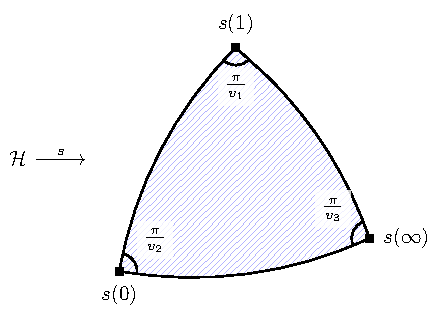
\includegraphics{pic/halfspace5.pdf}
		\end{minipage}
		\label{pic:Htriangle}
	\end{figure}
	
	通过Schwarz反射得到多值函数
	\begin{figure}[ht]
			\centering
			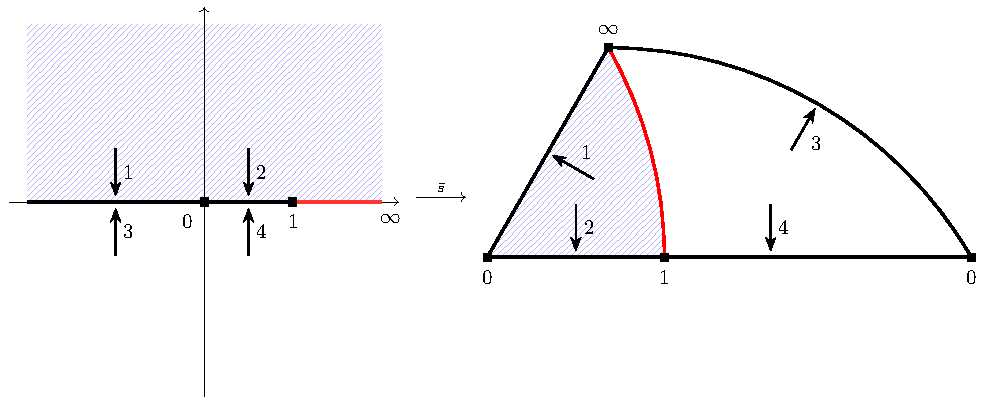
\includegraphics[width=.98\textwidth]{pic/halfspace4.pdf}
		\label{pic:Ctriangle}
	\end{figure}
	称其为\textbf{Schwarz $s$-函数},记作$ s(\frac{\pi}{v_1},\frac{\pi}{v_2},\frac{\pi}{v_3},J)$.
	%其中$\mathbb{PC}^1$, $\mathbb{C}^1$, $\mathcal{H}$为唯三的单连通Riemann面.
	容易得到,当$\frac{1}{v_1}+\frac{1}{v_2}+\frac{1}{v_3}>1$时, $\bar{s}^{-1}$为有理函数$\varPhi$;当$\frac{1}{v_1}+\frac{1}{v_2}+\frac{1}{v_3}=1$时, $\bar{s}^{-1}$为特殊的双周期函数;当$\frac{1}{v_1}+\frac{1}{v_2}+\frac{1}{v_3}=1$时, $\bar{s}^{-1}$为特殊的模函数.特别地,当$(v_1,v_2,v_3)=(2,3,\infty)$时, $\bar{s}^{-1}$与$j$-函数之间只差一个分式线性变换.
	
\end{remark}
\begin{exercise}
	当$(v_1,v_2,v_3)=(\infty,\infty,\infty)$时,情况如何?
\end{exercise}

利用Schwarz-Christoffe公式\cite[p237]{ahlfors1979complex},我们得到
$$z=\varPhi^{-1}(Z)=C \int_{0}^{Z} \omega^{-\beta_2} (\omega-1)^{-\beta_3}d \omega +C', \qquad \beta_i=1-\frac{1}{v_i}=\frac{v_i-1}{v_i}$$
由于$\varPhi$在$Z_0=0,1,\infty$\footnote{对$Z_0=\infty$,形式上将$1/Z$记作$Z-Z_0$,但本质上是一样的.}点处为分歧覆叠,记分歧指数为$v$,则在其附近,有
\begin{equation}
\begin{aligned}
Z-Z_0 = & f\left((z-z_0)^v\right), 	\qquad f(0) \neq 0 \\
z-z_0 = & \alpha (Z-Z_0)^{\frac{1}{v}}+ \beta (Z-Z_0)^{\frac{1}{v}} + \gamma (Z-Z_0)^{\frac{1}{v}} + \cdots 	\qquad \alpha \neq 0   \label{eq:expansion}
\end{aligned}
\end{equation}
代入$\varPhi$即可得到$\alpha,\beta,\gamma,\cdots$.

由构造, $\Gamma$将单值解析分支映至单值解析分支,越过支线所对应的分式线性变换亦可从图中看出.

记$\eta=\eta(Z)$为其中的一个解析分支, Schwarz导数$[f]_Z=\frac{f'''}{f'}-\frac{3}{2}\left(\frac{f''}{f'}\right)^2$.由于对任意$\gamma \in SL_2(\mathbb{R})$, $[\gamma(\eta)]_Z=[\eta]_Z$,故
$$[\varPhi^{-1}]_Z:\mathbb{PC}^1 \longrightarrow \mathbb{PC}^1 \qquad Z_0 \longmapsto [\eta]_Z(Z_0)$$
为良定义的亚纯函数,故为有理函数,记为$r(Z)$.
通过对\eqref{eq:expansion}计算,得到$r(Z)$具有形式\footnote{等式 $\displaystyle[Z^{\frac{1}{v}}]_Z=\frac{1-v^2}{2v^2Z^2}$可以揭示在展开时出现的首项系数.}
$$r(Z)=\frac{v_{1}^{2}-1}{2 v_{1}^{2}(Z-1)^{2}}+\frac{A}{Z-1}+\frac{v_{2}^{2}-1}{2 v_{2}^{2} Z^{2}}+\frac{B}{Z}+C_{3}$$
再将此形式在$\infty$处Laurent展开并对比,最终得到答案
$$r(Z)=\frac{v_{1}^{2}-1}{2 v_{1}^{2}(Z-1)^{2}}+\frac{v_{2}^{2}-1}{2 v_{2}^{2}Z^2} +\frac{\frac{1}{v_{2}^{2}}+\frac{1}{v_{2}^2}-\frac{1}{v_{3}^{2}}-1}{2(Z-1) Z}$$
故我们得到了解析分支$\eta$所满足的函数方程:
$$f'''f'-\frac{3}{2} (f'')^2-r(Z)(f')^2=0$$
非线性方程比线性方程总是要复杂一些.事实上,通过计算,我们总可以将$\eta$写为某个二阶线性方程的两个解$y_1,y_2$之商.
\section{预解式:近世代数视角}\label{sec:inverse-alge}

按照近世代数观点,将$\varPhi$视作有理函数,记
$$\varPhi(z)=\frac{f(z)}{g(z)}, \qquad f,g \text{ 互素}$$
寻找$\varPhi^{-1}(Z)$亦即方程$Zg(z)-f(z)=0 \;(\text{over }\mathbb{C}(Z))$的解.那么自然的流程如下:
\begin{itemize}
	\item 给出方程所对应的Galois群.
	\item 判定该方程是否有根式解:若有,具体解出;
	\item 在给出辅助方程后尝试解出(如预解式,模函数);\footnote{这是一个递归的过程,我们也会用这些方程来尝试解其他方程(如一般的五次方程)}
\end{itemize}
在Galois理论中,我们考虑域扩张$\mathbb{C}(z)/\mathbb{C}(Z)$所对应的Galois群
$$\Gal \left(\mathbb{C}(z)/\mathbb{C}(Z)\right) \subseteq \Aut_{\mathbb{C}}(\mathbb{C}(Z)) \overset{\sim}{\longrightarrow} \PSL_2(\mathbb{C})$$
由于对$\gamma \in \Gamma$, $\gamma z \in \mathbb{C}(z)$亦为方程的一个根,故$\mathbb{C}(z)$为$\mathbb{C}(Z)$关于多项式
$$p_W(T):= Zg(T)-f(T)$$
的分裂域, $\mathbb{C}(z)/\mathbb{C}(Z)$为Galois扩张, $\Gal\left(\mathbb{C}(z)/\mathbb{C}(Z)\right) \cong \Gamma$.

另外,我们有扩张与Galois群的反向对应:
\[	\setcounter{MaxMatrixCols}{15}
\begin{array}{ccccccccc|cc}
\mathbb{C}(z) &\supseteq &\mathbb{C}(Z_1^{(2)}) &\supseteq &\mathbb{C}(Z_2^{(2)}) &\supseteq &\mathbb{C}(Z_3) &\supseteq  &\mathbb{C}(Z_4) =  \mathbb{C}(Z_4') &\supseteq  &\mathbb{C}(Z_5)\\[-0.45cm]
&\underset{2}{}&&\underset{2}{}&&\underset{3}{}&&\underset{2}{}&&\underset{5}{}&\\
\{1\} &\lhd &C_2 &\lhd &D_2  &\lhd &A_4 &\lhd &S_4 &\leqslant &S_5
\end{array}
\]
竖线左边为根式扩张与正规子群序列的对应,右边为非循环单群($\Rightarrow$不可解群)与非分式扩张的对应.

为了进一步研究$A_5$,我们引入预解式的概念,希望在给出预解式某个根后得到方程$p_W(T)=0$的根:
\begin{defn}
	我们称$r \in K$相对于Galois扩张$K/k$的\textbf{预解式}(resolution)为$r$的最小多项式$R_{r,K/k}$.具体地,记$G:= \Gal(K/k)$, $H:= \Gal (k(r)/k)$,则$r$的预解式为
	$$R_{r,K/k}(T):= \prod_{\gamma \in G/H} (T-\gamma(r)) \in k[T]. $$
\end{defn}
\begin{example1}
	域扩张$\mathbb{Q}(\omega_5)/\mathbb{Q}$对应Galois群$(\mathbb{Z}/5\mathbb{Z})^{\times} =\mathbb{Z}/4\mathbb{Z}$,故
	$$R_{\omega_5, \mathbb{Q}(\omega_5)/\mathbb{Q}} (T)=(T-\omega_5)(T-\omega_5^2)(T-\omega_5^3)(T-\omega_5^4)=T^4+T^3+T^2+T+1$$
	$$R_{\omega_5+\omega_5^{-1}, \mathbb{Q}(\omega_5)/\mathbb{Q}} (T)=\left(T-(\omega_5+\omega_5^{-1})\right)\left(T-(\omega_5^2+\omega_5^{-2})\right)=T^2+T-1$$
	观察: $\omega_5+\omega_5^{-1}=2\cos 72^{\circ} =\frac{1}{2}(\sqrt{5}-1)$为方程$T^2+T-1=0$的根.
\end{example1}
\begin{example1}
	运用\cite[p46-47]{klein2003lectures}的数据及表\ref{tb:equations}中的辅助方程,我们得到
	\begin{equation*}
	\begin{aligned}
	R_{z,\mathbb{C}(z)/\Cln}(T)=\;& (T-z)(T-\omega_{n}z)\cdots (T-\omega_{n}^{n-1}z)\\
	=\;&T^n-z^n\\
	R_{\Cnoln, \Cln/\Clln}(T)=\;& \left(T-Z_1^{(n)}\right)\left(T-\frac{1}{Z_1^{(n)}}\right)\\
	=\;&T^2+\left(4Z_2^{(n)}-2\right)T+1\\	R_{\Cnolll,\Clll/\mathbb{C}(Z_3)}(T)=\;& \left(T-Z_2^{(2)}(z)\right)\left(T-Z_2^{(2)}\left(i\frac{z+1}{z-1}\right)\right)\left(T-Z_2^{(2)}\left(\frac{z+i}{z-i}\right)\right)\\
	=\;& \left(T-Z_2^{(2)}\right)\left(T+\frac{1}{Z_2^{(2)}+1}\right)\left(T+\frac{Z_2^{(2)}+1}{Z_2^{(2)}}\right)\\
	=\;& T^3+3\omega_3 \frac{Z_3-\omega_3}{Z_3-1}T^2+3\omega_3^2 \frac{Z_3-\omega_3^2}{Z_3-1}T+1\\
	R_{Z_3,\mathbb{C}(Z_3)/\mathbb{C}(Z_4)}(T)=\;& \left(T-Z_3\right)\left(T-\frac{1}{Z_3}\right)\\
	=\;&T^2-\left(\frac{4}{Z_4^{(n)}}+2\right)T+1\\
	\end{aligned}
	\end{equation*}
	如果想偷懒,直接对表\ref{tb:equations}中的辅助方程做变换即可,如:
	$$R_{Z_4',\mathbb{C}(Z_4)/\mathbb{C}(Z_5)}(T)=\;(T-3)^3(T^2-11T+64)+1728Z_5 $$
\end{example1}
对$t',W'$配凑正十二面体的不变轨道$H,\mathcal{T},f$后得到亚纯函数
$$u:=\frac{12f^2}{\mathcal{T}} \cdot t' \qquad v:=\frac{12f}{H} \cdot W'$$
我们想计算预解式$R_{u,\mathbb{C}(Z_4)/\mathbb{C}(Z_5)}$和$R_{v,\mathbb{C}(Z_4)/\mathbb{C}(Z_5)}$,为了方便计算(形式比不变函数更易计算),我们引入形式预解式的概念:
\begin{defn}
	对形式$F \in \mathbb{C}\homopoly$,记
	$$\Gamma_F':= \left\{ \gamma' \in \Gamma'|F \circ \gamma' = F \right\} \leqslant \Gamma'$$
	$F$的\textbf{形式预解式}(form resolution)定义为
	$$R_F(T):= \prod_{\gamma' \in \Gamma' / \Gamma'_F}(T-F \circ \gamma') 	\quad \in \mathbb{C}[H,\mathcal{T},f]$$
\end{defn}
\begin{example1}
	直接计算/对多项式系数进行分析得到\footnotemark.
	$$R_{t'}(T)=T^5-10fT^3+45f^2T-\mathcal{T}$$
	$$R_{W'}(T)=T^5+40f^2T^2-5fHT+H^2$$
\end{example1}

\footnotetext{具体细节可见\cite[p112-116]{klein2003lectures}或\cite[Chapter 4.8]{shurman1997geometry}}
通过代数变换$\left(\displaystyle Z_5':= \frac{1}{1728(1-Z_5)},Z_5':= \frac{1}{1728(1-Z_5)}\right)$,得到预解式
$$R_{u,\mathbb{C}(Z_4)/\mathbb{C}(Z_5)}(T):=T^5-10Z_5'T^3+45{Z_5'}^2T-{Z_5'}^2$$
$$R_{v,\mathbb{C}(Z_4)/\mathbb{C}(Z_5)}(T):=T^5+40Z_5''T^2-5Z_5''T+Z_5''$$
其中$R_{u,\mathbb{C}(Z_4)/\mathbb{C}(Z_5)}(T)$被称作\textbf{Brioschi预解式}.固定$Z_5=\lambda_0$,若给出$R_{u,\mathbb{C}(Z_4)/\mathbb{C}(Z_5)}(T)=0$的一个解$T=u_0$,则由exercise \ref{exercise:function},我们得到
$$Z_4'=\frac{t'^2}{f}=\frac{u_0^2\mathcal{T}^2}{144f^5}=12u_0^2(1-Z_5)$$
从而依次解出$Z_4,Z_3,Z_2^{(2)},Z_1^{(2)},z$,得到方程$Z_5(z)=\lambda_0$的解.因此,解正十二面体方程等价于解如下五次方程:
\begin{equation}\label{eq:brioschi}
T^5-10\lambda T^3 +45\lambda^2T-\lambda^2=0	\qquad \text{其中$\lambda$为未定元}
\end{equation}
在下一节中,我们将尝试考察一般的五次方程,将其等价于对方程\eqref{eq:brioschi}的求解.
\section{一元五次方程的解}
本节开始着手一元五次方程的解.本节的目标是将一般的五次方程化归为方程\eqref{eq:brioschi}或
\begin{equation}\label{eq:Bring-Jarrard}
x^5-x+\gamma=0
\end{equation}
的形式.我们主要讨论域为复数域的情况,并在注记中提及一般域时需要额外考虑的情况.

在这个过程中我们将不加说明地使用初等对称多项式、Newton恒等式与结式的相关知识,需要的读者可查阅\cite[Chapter 5.1-5.3]{shurman1997geometry}.

同低次方程的解类似,任一个一元五次方程均可以化为下列形式\footnote{这里假设域的特征不为2,3.}:
\begin{equation}\label{eq:firstreduction}
x^5+5\alpha x^2+5 \beta x+\gamma=0
\end{equation}
\begin{remarks}\
	\begin{itemize}
		\item 在这个过程中我们已经隐式使用了Jerrard-Bring约化.设原方程为
		$$f(x):=x^5+a_4x^4+a_3x^3+a_2x^2+a_1x+a_0=0$$
		通过设$x'=x+b_0$我们消去$a_4$,再通过设$x'=x^2+b_1x+b_0$消去$a_3$.
		\item 注意我们在消去$a_3$时得到关于$b_2$的一个二次方程,故变换的时候$b_2$可能超出我们所考虑的域.具体来说,取基域$k:=\mathbb{C}[a_4,a_3,\ldots,a_0]$,扩域$K$为$k$在方程$f(x)=0$下的分裂域,则我们得到的$b_2$很可能不属于$K$.为此,我们将$b_2$同时添入基域$k$与扩域$K$.可以证明,添根在大多数情况下\footnote{如当变换$x'=x^2+b_1x+b_0$将方程$f(x)$的根映至不同值时,此时称该变换为非退化的.其他情况将有效将方程降次.}均不改变对应的Galois理论,如图所示:
		
		\begin{figure}[ht]
			
			\begin{minipage}[t]{.9\textwidth}
				\vspace{0.1cm}
				\centering
				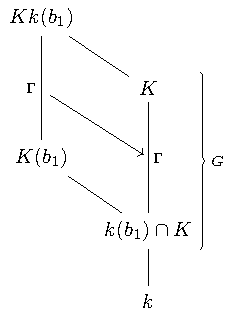
\includegraphics{commu/commu3.pdf}
				
			\end{minipage}
			\label{pic:galois}
		\end{figure}
		
		
		\item 这个方程的根$[r_1:r_2:\cdots:r_5]$显然落在二次曲面
		$$\mathcal{Q}:=\left\{[r_1:r_2:\cdots:r_5] \in \mathbb{PC}^4 \,\middle|\, \sum_{i=1}^{5}r_i=\sum_{i=1}^{5}r_i^2=0 \right\}$$
		中.由于它是$\mathbb{PC}^3$中的满秩曲面,故同构于$\mathbb{PC}^1 \times \mathbb{PC}^1$.另外我们也有三次曲面
		$$\mathcal{C}:=\left\{[r_1:r_2:\cdots:r_5] \in \mathbb{PC}^4 \,\middle|\, \sum_{i=1}^{5}r_i=\sum_{i=1}^{5}r_i^3=0 \right\},$$
		这两个曲面在约化过程中将起到重大作用,尤其是曲面$\mathcal{Q}$.
	\end{itemize}
\end{remarks}

若通过更进一步的Jerrard-Bring约化,则可以通过解额外的辅助方程\footnote{参见\cite{green1978on},自然仍需添入额外的二次/三次根.}将方程\eqref{eq:firstreduction}化为
$$x^5-x+\gamma=0 \quad \text{or} \quad x^5+\gamma=0\;\text{(easy!)}$$
的形式,前一种被称为Bring-Jarrard form,此为一路.

另外一路,我们将按照\cite[5.8]{shurman1997geometry}的流程,将方程\eqref{eq:firstreduction}化为\eqref{eq:brioschi}的形式.设原方程为
$$p(T):=T^5-\sigma_3 T^2+\sigma_4 T -\sigma_5$$
通过定义满足一定限制的多项式$t(T) \in k[T] \; \big(\hspace{-0.25cm}\mod p(T)\big)$,我们得到新的五次方程
\begin{equation}\label{eq:closetoBri}
q(T):=\prod_{i=1}^{5} (T-t(r_i))=T^5+d_1T^4+d_2T^3+d_3T^2+d_4T+d_5 \in k[T]
\end{equation}
简化后得到Brioschi预解式.这个过程的难点在于复杂的代数构造:
\begin{enumerate}[Step 1.]
	\item 构造三次或四次首一多项式$\psi(T) \in k[T]$,使得\footnote{主要的思路是配凑,可参见\cite[exercise 5.8.1]{shurman1997geometry}}
	$$\sum \psi(r_i)=\sum \psi(r_i)^2=\sum r_i\psi(r_i)=0$$
	这样我们才能令$\mathbb{C}^2$以如下方式作用于曲面$\mathcal{Q}$:
	$$(a,b) \longmapsto [r_i \mapsto ar_i+b\psi(r_i)]$$
	\item 将域$k[T]/(p(T))$视作5维$k$-线性空间,则$T^2,\psi(T) T ,\psi(T)^2, T,\psi(T),1$线性相关,故有非零等式
	$$\alpha T^2+2\beta T \psi +\gamma \psi^2 -aT-b\psi+c=0 	\qquad \text{in $k[T]$}$$
	通过代入$T=r_i$后求和得到$c=0$,从而令
	\begin{equation*}
	\begin{aligned}
	L(X,Y):=&\,aX+bY=\begin{pmatrix}
	a&b
	\end{pmatrix}
	\begin{pmatrix}
	X\\Y
	\end{pmatrix}\\
	Q(X,Y):=&\,\alpha X^2+2\beta XY+\gamma Y^2=\begin{pmatrix}
	X & Y
	\end{pmatrix}
	\begin{pmatrix}
	\alpha & \beta\\
	\beta & \gamma
	\end{pmatrix}
	\begin{pmatrix}
	X \\ Y
	\end{pmatrix}
	\end{aligned}
	\end{equation*}
	我们得到
	\begin{itemize}
		\item $L(T,\psi(T))\equiv Q(T,\psi(T)) \quad \text{mod } p(T)$
		\item $L,Q$均不为$0$多项式,且$L(T,\psi(T))\equiv Q(T,\psi(T)) \neq 0 \quad \text{mod } p(T)$.
		\item $L \nmid Q \text{ in }k[X,Y]$ 
		\item $m:=Q(b,-a), \quad \delta:=\alpha\gamma-\beta^2$均不为零.
	\end{itemize}
	\item 先承认一个引理:
	\begin{lemma}\label{lem:matrixproof}
		设$L$, $Q$, $m$, $\delta$如上所示,且$L \nmid Q$.那么,存在单项式$\tilde{L}:=\tilde{a}X+\tilde{b}Y \in k[X,Y]$,使得
		\begin{equation}\label{eq:matrixproof}
		mQ(X,Y)=\tilde{L}(X,Y)^2+\delta L(X,Y)^2.
		\end{equation}
	\end{lemma}
	作为推论,我们有
	$$mL \equiv mQ =\tilde{L}^2 +\delta L^2=(\tilde{L}+\sqrt{-\delta}L)(\tilde{L}-\sqrt{-\delta}L) 	\qquad \text{in }k(\sqrt{-\delta})[T]$$
	在这之后我们终于可以给出多项式$t(T):=\tilde{L}(T,\psi(T)) \cdot L^{-1}(T,\psi(T))$(在模$p$意义下),且$t$满足
	\begin{equation*}
	\begin{aligned}
	t\equiv (1+\sqrt{-\delta}L_1)L_1^{-1} \; \text{ mod }p \qquad L_1:=(\tilde{L}+\sqrt{-\delta}L)/m\\
	t\equiv (1-\sqrt{-\delta}L_2)L_2^{-1} \; \text{ mod }p \qquad L_2:=(\tilde{L}-\sqrt{-\delta}L)/m\\
	\end{aligned}
	\end{equation*}
	\item 我们验证多项式\eqref{eq:closetoBri}即是我们所求的多项式.由于
	$$0=q\big(t(r_i)\big)=q\big(t(L_1(r_i))\big)=q(L_1)\big(r_i\big),$$
	展开得到
	$$L_1^5q(L_1)= \Big((1+\sqrt{-\delta}L_1)^5+d_1 L_1 (1+\sqrt{-\delta}L_1)^4 + \cdots + d_5 L_1^5\Big)$$
	中的$3$, $4$次系数均为$0$,由此得到多项式$q$系数的$2$个线性函数.对$q(L_2)$采用同样的操作,解完方程组后得到
	$$q=T^5+\frac{10}{3}\delta T^3+5\delta^2T+d_5$$
	最后令$\displaystyle S:=-\frac{\delta^2}{9d_5}T$, $\;\displaystyle W:=-\frac{\delta^5}{3^5 \cdot d_5^2}$,得到Brioschi预解式:
	$$q(S)=S^5-10WS^3+45W^2S-W^2$$
	\item \begin{proof}[引理\ref{lem:matrixproof}的证明]\
		假设我们已经找出$\tilde{L}$,将方程写成矩阵形式:
		\begin{equation*}
		\begin{aligned}
		mQ(X,Y)=&\tilde{L}(X,Y)^2+\delta L(X,Y)^2\\
		\Longleftrightarrow\; m\begin{pmatrix}
		\alpha & \beta \\ \beta & \gamma
		\end{pmatrix}=&
		\begin{pmatrix}
		\tilde{a} \\ \tilde{b}
		\end{pmatrix}
		\begin{pmatrix}
		\tilde{a} & \tilde{b}
		\end{pmatrix}
		+\delta
		\begin{pmatrix}
		a \\ b
		\end{pmatrix}
		\begin{pmatrix}
		a & b
		\end{pmatrix}\\
		=& 
		\begin{pmatrix}
		\tilde{a} & a \\ \tilde{b} & b
		\end{pmatrix}
		\begin{pmatrix}
		1 & 0 \\ 0 & \delta
		\end{pmatrix}
		\begin{pmatrix}
		\tilde{a} & \tilde{b} \\ a & b
		\end{pmatrix}
		\end{aligned}
		\end{equation*}
		取$\tilde{a}:=a\beta-b\alpha$, $\tilde{b}:=a\gamma-b\beta$即可满足条件.
	\end{proof}
\end{enumerate}


\section{通过模形式解五次方程}
若是只要求形式幂级数解,则对方程\eqref{eq:Bring-Jarrard}有一个组合得到的解:
$$x(\gamma) = \sum_{k=0}^{\infty} \binom{5k}{k} \frac{\gamma^{4k+1}}{4k+1}$$
那么我们的故事就结束了.不过,这样直接的解总是显得不太自然.或者说,这不过是为路人提供的人为捷径,而真正的探险者则有意避开,为的就是在那危峰兀立的山崖上,瞥见常人所不能识的自然之美.
%如果你愿意追随,那么,我们将会用正二十面体方程来解一般的五次方程(or 将一般的五次方程化为正二十面体方程),再用模形式来解正二十面体方程.这样看,正二十面体方程则是五次方程的一个``典型代表",而它的模形式解则不过是图\ref{fig:tran}中辅助方程的一个类比.

记$$\Gamma(N):=\left\{ \begin{pmatrix}
a &b \\ c & d
\end{pmatrix} \in SL_2(\mathbb{Z}) \;\middle|\; \begin{pmatrix}
a &b \\ c & d
\end{pmatrix} \equiv \begin{pmatrix}
1 &0 \\ 0 & 1
\end{pmatrix} \mod N  \right\}$$
特别地, $\Gamma(1)=SL_2(\mathbb{Z})$,我们有正合列

\begin{center}
	\begin{tikzcd}
		1 \arrow[r]           & \Gamma(5) \arrow[r]             & PSL_2(\mathbb{Z}) \arrow[r]   & PSL_2(\mathbb{F}_5) \arrow[d, "\sim"] \arrow[r] & 1 \\
		&                  &     & {\Gamma_{(2,3,5)}}                              &   \\
		\mathcal{H} \arrow[r] & \mathcal{H}/\Gamma(5) \arrow[r] & \mathcal{H}/\Gamma(1) &                                                 &  
	\end{tikzcd}
\end{center}
\vspace{-2cm}\text{从而得到}\\[1.5cm]
诱导的交换图($\mathcal{H}^*:=\mathcal{H} \cup \mathbb{Q}^*$)

\begin{center}
	\begin{tikzcd}
		\mathcal{H}^* \arrow[r, "r"] & \mathcal{H}^*/\Gamma(5) \arrow[r, "\pi_1"] \arrow[d, "\hat{j}_5","\sim"'] & \mathcal{H}^*/\Gamma(1) \arrow[d, "\hat{j}","\sim"'] \\
		& \mathbb{PC}^1 \arrow[r, "I"]                                      & \mathbb{PC}^1                               
	\end{tikzcd}
\end{center}
我们留给下一章的任务:
\begin{enumerate}
	\item 构造$j_5:\mathcal{H}^* \longrightarrow \mathbb{PC}^1 $,证明其诱导的$\hat{j}_5:\mathcal{H}^*/\Gamma(5) \longrightarrow \mathbb{PC}^1$为同构;
	\item 构造$I:= \hat{j} \circ \pi_1 \circ \hat{j}_5^{-1}$,验证其满足$I=1728Z_5$,从而得到
	$$Z_5^{-1}=\frac{1}{1728}I^{-1}=\frac{1}{1728}j_5 \circ j^{-1}$$
	从而通过模方程$j(\tau)=j_0$的解得到正二十面体方程的解.
\end{enumerate}